
\documentclass[12pt]{article}
\usepackage[margin=1in]{geometry}
\usepackage{amsmath, amssymb}
\usepackage{tikz}
\usepackage{xcolor}
\usepackage{wrapfig}
\usepackage{multicol}
\usepackage{mathpazo} % Elegant font
\linespread{1.1}      % Slightly looser line spacing

\definecolor{headerblue}{rgb}{0.0, 0.6, 0.9}

\begin{document}

\begin{figure}[h!]
    \begin{minipage}{0.45\textwidth}  % Set the width of the image
            \includegraphics[width=\textwidth]{/storage/emulated/0/vinod/IMG-20250515-WA0024.png}  % Replace 'image.png' with your image file name
	        \end{minipage} \hfill
		    \begin{minipage}{0.45\textwidth}  % Set the width of the text block
		            \textbf{Name :Kiran Kumar Reddy L} \\
			            \textbf{Batch:2} \\
				            \textbf{ID   :cometfwc027} \\
					            \textbf{Date :16th may 2025} 
						        \end{minipage}
							\end{figure}

% Header
\noindent
\textcolor{headerblue}{\textbf{178}} \hfill 
\vspace{-9pt}
\textcolor{headerblue}{\textbf{Mathematics}} \\
\textcolor{headerblue}{\rule{\textwidth}{2pt}}

\vspace{0.8em}
\noindent
\textbf{\textcolor{headerblue}{Remark:}} Since the hypotenuse is the longest side in a right triangle, the value of $\sin A$ or $\cos A$ is always less than 1 (or, in particular, equal to 1).

\vspace{0.8em}
\noindent
Let us consider some examples.

\begin{wrapfigure}{r}{0.4\textwidth}
\vspace{-3.5em}
\centering
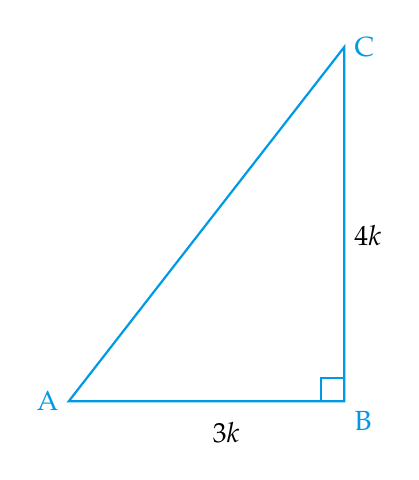
\begin{tikzpicture}[scale=1]
\draw[thick, color=headerblue] (-0.5,0) node[left] {A} -- (3,0) node[below right] {B} -- (3,4.5) node[right] {C} -- cycle;
\draw[thick,color=headerblue] (3,0) ++(-0.3,0) -- ++(0,0.3) -- ++(0.3,0);
\node at (1.5, -0.4) {$3k$};
\node at (3.3, 2.1) {$4k$};
\end{tikzpicture}

\textcolor{headerblue}{Fig. 8.8}
\end{wrapfigure}

\vspace{1em}
\noindent
\textbf{\textcolor{headerblue}{Example 1:}} Given $ \tan A = \dfrac{4}{3}$, find the other trigonometric ratios of the angle $A$.

\vspace{0.5em}
\noindent
\textbf{\textcolor{headerblue}{Solution:}}\noindent Let us first draw a right $\triangle ABC$ (see Fig. 8.8).

\vspace{0.5em}
\noindent
Now, we know that $\tan A = \dfrac{BC}{AB} = \dfrac{4}{3}$. \\
Therefore, if $BC = 4k$, then $AB = 3k$, where $k$ is a positive number.

\vspace{0.5em}
\noindent
Now, by using the Pythagoras Theorem, we have
\[
AC^2 = AB^2 + BC^2 = (3k)^2 + (4k)^2 = 25k^2
\quad \Rightarrow \quad
AC = 5k
\]

\vspace{0.5em}
\noindent
Now, we can write all the trigonometric ratios using their definitions:
\begin{align*}
\sin A &= \dfrac{BC}{AC} = \dfrac{4k}{5k} = \dfrac{4}{5}, \\
\cos A &= \dfrac{AB}{AC} = \dfrac{3k}{5k} = \dfrac{3}{5}
\end{align*}

\vspace{-0.5em}
\noindent
Therefore, \quad
$\cot A = \dfrac{1}{\tan A} = \dfrac{3}{4}, \quad 
\csc A = \dfrac{1}{\sin A} = \dfrac{5}{4}, \quad 
\sec A = \dfrac{1}{\cos A} = \dfrac{5}{3}$

\vspace{1em}

\begin{wrapfigure}{r}{0.58\textwidth}
\vspace{-2em}
\centering
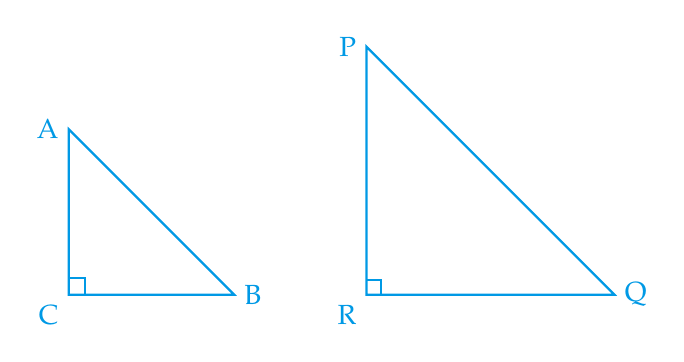
\begin{tikzpicture}[scale=0.7]
% Triangle ABC
\draw[thick, color=headerblue] (0,0) node[right] {B} -- (-3,0) node[below left] {C} -- (-3,3) node[left] {A} -- cycle;
\draw[thick,color=headerblue] (-3,0) ++(0.3,0) -- ++(0,0.3) -- ++(-0.3,0);

% Triangle PQR shifted to right
\begin{scope}[xshift=6cm,scale=0.9]
\draw[thick, color=headerblue] (1,0) node[right] {Q} -- (-4,0) node[below left] {R} -- (-4,5) node[left] {P} -- cycle;
\draw[thick,color=headerblue] (-4,0) ++(0.3,0) -- ++(0,0.3) -- ++(-0.3,0);
\end{scope}
\end{tikzpicture}

\textcolor{headerblue}{\textbf{Fig. 8.9}}
\end{wrapfigure}

\vspace{1em}
\noindent
\textbf{\textcolor{headerblue}{Example 2:}} If $\angle B$ and $\angle Q$ are acute angles such that $\sin B = \sin Q$, then prove that $\angle B = \angle Q$.

\vspace{0.5em}
\noindent
\textbf{\textcolor{headerblue}{Solution:}} Let us consider two right triangles $ABC$ and $PQR$ where $\sin B = \sin Q$ (see Fig. 8.9).
\[\]


\centerline{2019-2020}

\newpage
\noindent
\textcolor{headerblue}{\textbf{179}} \hfill 
\vspace{-9pt}
\textcolor{headerblue}{\textbf{Introduction to Trigonometry}} \\
\textcolor{headerblue}{\rule{\textwidth}{1pt}}

\vspace{1em}
\[
\sin B = \frac{AC}{AB}
\]
We have
\[
\sin Q = \frac{PR}{PQ}
\]

\noindent Then \hfill $\dfrac{\mathrm{AC}}{\mathrm{AB}} = \dfrac{\mathrm{PR}}{\mathrm{PQ}}$ \hfill \phantom{(0)}

\vspace{1em}

\noindent Therefore, \hfill $\dfrac{\mathrm{AC}}{\mathrm{PR}} = \dfrac{\mathrm{AB}}{\mathrm{PQ}} = k, \text{ say}$ \hfill $(1)$

\vspace{1em}

\noindent Now, using Pythagoras theorem, \[\mathrm{BC} = \sqrt{\mathrm{AB}^2 - \mathrm{AC}^2}\]
\noindent and 
\[\mathrm{QR} = \sqrt{\mathrm{PQ}^2 - \mathrm{PR}^2}\]

\vspace{1em}

\noindent So, \quad \quad \quad $\dfrac{\mathrm{BC}}{\mathrm{QR}} = \dfrac{\sqrt{\mathrm{AB}^2 - \mathrm{AC}^2}}{\sqrt{\mathrm{PQ}^2 - \mathrm{PR}^2}} = \dfrac{\sqrt{k^2\mathrm{PQ}^2 - k^2\mathrm{PR}^2}}{\sqrt{\mathrm{PQ}^2 - \mathrm{PR}^2}} = \dfrac{k\sqrt{\mathrm{PQ}^2 - \mathrm{PR}^2}}{\sqrt{\mathrm{PQ}^2 - \mathrm{PR}^2}} = k$ \hfill $(2)$

\vspace{1em}

\noindent From (1) and (2), we have \[ \dfrac{\mathrm{AC}}{\mathrm{PR}} = \dfrac{\mathrm{AB}}{\mathrm{PQ}} = \dfrac{\mathrm{BC}}{\mathrm{QR}}\]\

\vspace{1em}

\noindent Then, by using Theorem 6.4, $\triangle \mathrm{ACB} \sim \triangle \mathrm{PRQ}$ and therefore, $\angle \mathrm{B} = \angle \mathrm{Q}$.

\vspace{2em}
\noindent
\textbf{\textcolor{headerblue}{Example 5:}} In $\triangle OPQ$, right-angled at $P$,
\newline
$OP = 7\,\text{cm}$ and $OQ - PQ = 1\,\text{cm}$ (see Fig. 8.12). \\
Determine the values of $\sin Q$ and $\cos Q$.



\vspace{0.5em}
\noindent
\textbf{\textcolor{headerblue}{Solution:}} In $\triangle OPQ$, we have:

\newpage
\noindent
\textcolor{headerblue}{\textbf{178}} \hfill 
\vspace{-9pt}
\textcolor{headerblue}{\textbf{Mathematics}} \\
\textcolor{headerblue}{\rule{\textwidth}{2pt}}

\begin{wrapfigure}{r}{0.2\textwidth}
\vspace{-1em}
\centering
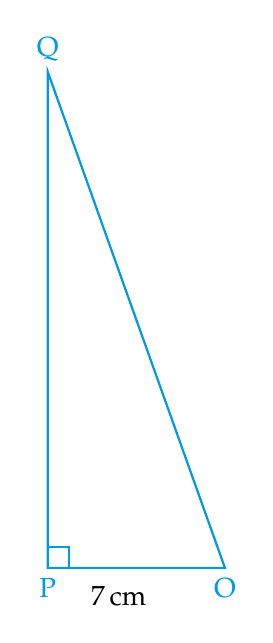
\begin{tikzpicture}[scale=0.9]
\draw[thick, color=headerblue] (-1,0) node[below] {O} -- (-3.5,0) node[below] {P} -- (-3.5,7) node[above] {Q} -- cycle;
\draw[thick,color=headerblue] (-3.5,0) ++(0.3,0) -- ++(0,0.3) -- ++(-0.3,0);
\node at (-2.5, -0.4) {$7\,\text{cm}$};
\end{tikzpicture}

\textcolor{headerblue}{\textbf{Fig. 8.12}}
\end{wrapfigure}

\begin{align*}
    & OQ^2 = OP^2 + PQ^2 \\
    \text{i.e.,} \qquad \qquad \qquad \qquad & (1 + PQ)^2 = OP^2 + PQ^2 \qquad \qquad \text{(Why?)} \\
    \text{i.e.,} \qquad \qquad \qquad \qquad & 1 + PQ^2 + 2PQ = OP^2 + PQ^2 \\
    \text{i.e.,} \qquad \qquad \qquad \qquad & 1 + 2PQ = 7^2 \qquad \qquad \qquad \qquad \quad \text{(Why?)} \\
    \text{i.e.,} \qquad \qquad \qquad \qquad & 2PQ = 49 - 1 = 48 \\
    \text{i.e.,} \qquad \qquad \qquad \qquad & PQ = 24\,\text{cm}\quad\text{and}\quad OQ = 1 + PQ = 25\,\text{cm} \\
\end{align*}

\quad\text{So}, \qquad \qquad \qquad \qquad $\displaystyle \sin Q = \dfrac{7}{25}$ \quad and \quad $\displaystyle \cos Q = \dfrac{24}{25}$
\vspace{0.5em}

\centerline{2019-2020}

\end{document}
